\documentclass{standalone}
\usepackage{tikz}
\usetikzlibrary{patterns, positioning}


\begin{document}
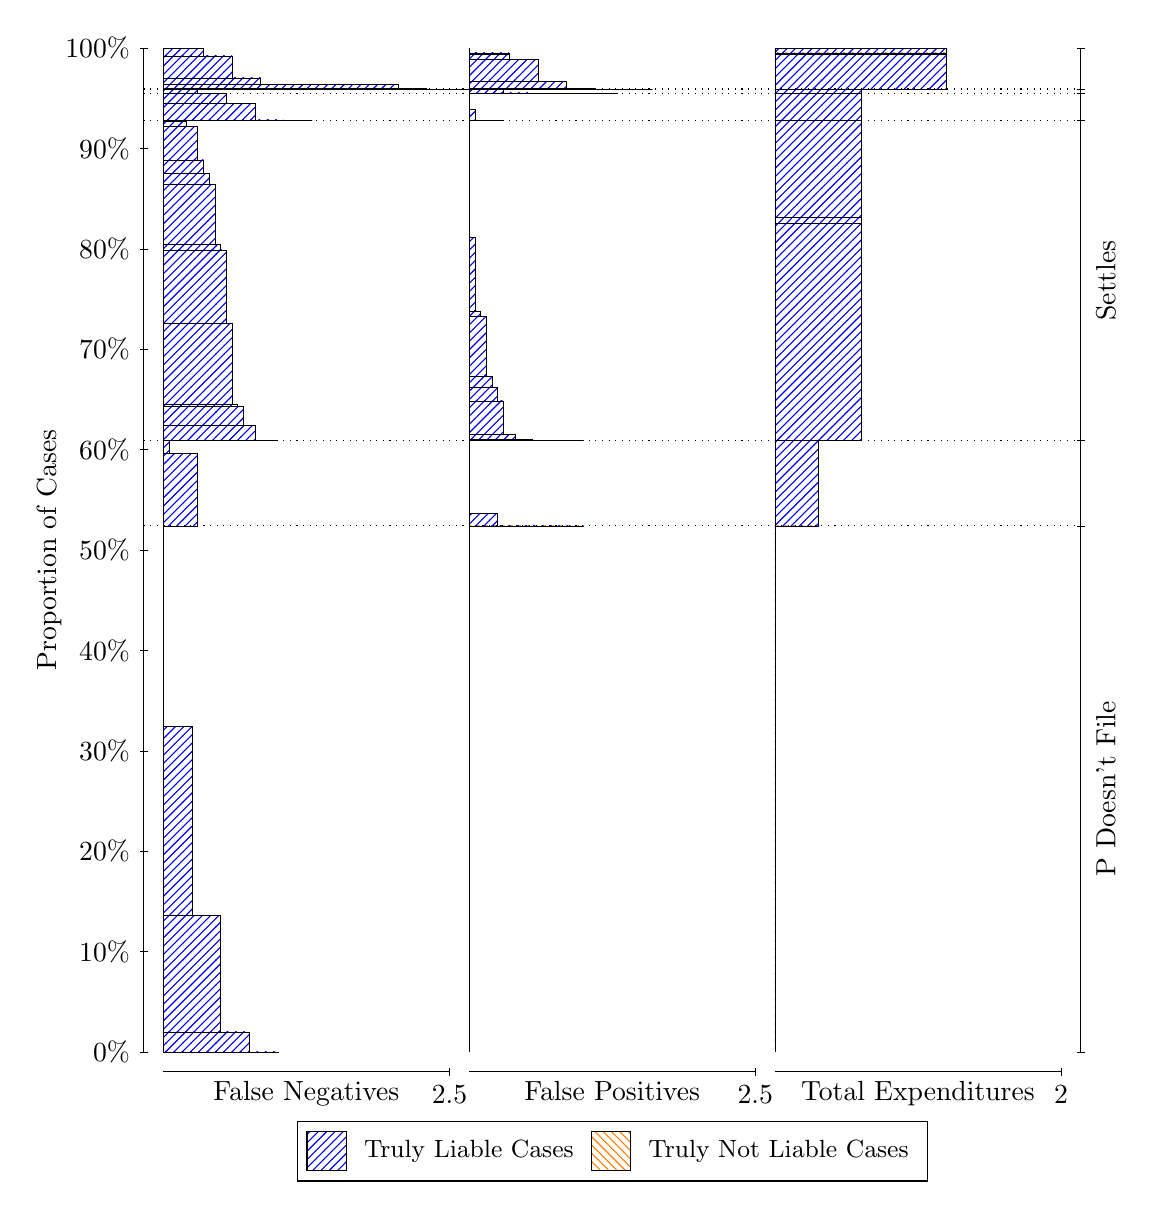
\begin{tikzpicture}
\draw[black, very thin] (1.5,1.75) -- (1.5,14.5);
\node[rotate=90, text=black, anchor=center] at (0.3, 8.125) {Proportion of Cases};
\draw[black, very thin] (1.45,1.75) -- (1.55,1.75);
\node[text=black, anchor=east] at (1.45, 1.75) {0\%};
\draw[black, very thin] (1.45,3.025) -- (1.55,3.025);
\node[text=black, anchor=east] at (1.45, 3.025) {10\%};
\draw[black, very thin] (1.45,4.3) -- (1.55,4.3);
\node[text=black, anchor=east] at (1.45, 4.3) {20\%};
\draw[black, very thin] (1.45,5.575) -- (1.55,5.575);
\node[text=black, anchor=east] at (1.45, 5.575) {30\%};
\draw[black, very thin] (1.45,6.85) -- (1.55,6.85);
\node[text=black, anchor=east] at (1.45, 6.85) {40\%};
\draw[black, very thin] (1.45,8.125) -- (1.55,8.125);
\node[text=black, anchor=east] at (1.45, 8.125) {50\%};
\draw[black, very thin] (1.45,9.4) -- (1.55,9.4);
\node[text=black, anchor=east] at (1.45, 9.4) {60\%};
\draw[black, very thin] (1.45,10.675) -- (1.55,10.675);
\node[text=black, anchor=east] at (1.45, 10.675) {70\%};
\draw[black, very thin] (1.45,11.95) -- (1.55,11.95);
\node[text=black, anchor=east] at (1.45, 11.95) {80\%};
\draw[black, very thin] (1.45,13.225) -- (1.55,13.225);
\node[text=black, anchor=east] at (1.45, 13.225) {90\%};
\draw[black, very thin] (1.45,14.5) -- (1.55,14.5);
\node[text=black, anchor=east] at (1.45, 14.5) {100\%};

\draw[black, very thin] (13.4,1.75) -- (13.4,14.5);
\draw[black, very thin] (13.35,1.75) -- (13.45,1.75);
\node[anchor=west] at (13.35, 1.75) {};
\draw[black, very thin] (13.35,8.4315) -- (13.45,8.4315);
\node[anchor=west] at (13.35, 8.4315) {};
\draw[black, very thin] (13.35,9.5172) -- (13.45,9.5172);
\node[anchor=west] at (13.35, 9.5172) {};
\draw[black, very thin] (13.35,13.582) -- (13.45,13.582);
\node[anchor=west] at (13.35, 13.582) {};
\draw[black, very thin] (13.35,13.928) -- (13.45,13.928);
\node[anchor=west] at (13.35, 13.928) {};
\draw[black, very thin] (13.35,13.979) -- (13.45,13.979);
\node[anchor=west] at (13.35, 13.979) {};
\draw[black, very thin] (13.35,14.5) -- (13.45,14.5);
\node[anchor=west] at (13.35, 14.5) {};

\draw[black, very thin, pattern color=blue, pattern=north east lines] (1.75,1.75) rectangle (3.2033,1.7525);
\draw[black, very thin, pattern color=blue, pattern=north east lines] (1.75,1.7525) rectangle (2.84,2.0051);
\draw[black, very thin, pattern color=blue, pattern=north east lines] (1.75,2.0051) rectangle (2.4767,3.4891);
\draw[black, very thin, pattern color=blue, pattern=north east lines] (1.75,3.4891) rectangle (2.1133,5.883);
\draw[black, very thin, pattern color=orange, pattern=north west lines] (1.75,5.883) rectangle (1.75,5.883);
\draw[black, very thin, pattern color=blue, pattern=north east lines] (1.75,5.883) rectangle (1.75,8.4315);
\draw[black, very thin, pattern color=blue, pattern=north east lines] (1.75,8.4315) rectangle (2.186,9.3557);
\draw[black, very thin, pattern color=blue, pattern=north east lines] (1.75,9.3557) rectangle (1.8227,9.5166);
\draw[black, very thin, pattern color=orange, pattern=north west lines] (1.75,9.5166) rectangle (1.75,9.5166);
\draw[black, very thin, pattern color=blue, pattern=north east lines] (1.75,9.5166) rectangle (1.75,9.5172);
\draw[black, very thin, pattern color=blue, pattern=north east lines] (1.75,9.5172) rectangle (3.2033,9.5172);
\draw[black, very thin, pattern color=blue, pattern=north east lines] (1.75,9.5172) rectangle (3.058,9.5172);
\draw[black, very thin, pattern color=blue, pattern=north east lines] (1.75,9.5172) rectangle (2.9127,9.7084);
\draw[black, very thin, pattern color=blue, pattern=north east lines] (1.75,9.7084) rectangle (2.84,9.7121);
\draw[black, very thin, pattern color=blue, pattern=north east lines] (1.75,9.7121) rectangle (2.7673,9.9505);
\draw[black, very thin, pattern color=blue, pattern=north east lines] (1.75,9.9505) rectangle (2.6947,9.9733);
\draw[black, very thin, pattern color=blue, pattern=north east lines] (1.75,9.9733) rectangle (2.622,11.006);
\draw[black, very thin, pattern color=blue, pattern=north east lines] (1.75,11.006) rectangle (2.5493,11.936);
\draw[black, very thin, pattern color=blue, pattern=north east lines] (1.75,11.936) rectangle (2.4767,12.007);
\draw[black, very thin, pattern color=blue, pattern=north east lines] (1.75,12.007) rectangle (2.404,12.773);
\draw[black, very thin, pattern color=blue, pattern=north east lines] (1.75,12.773) rectangle (2.3313,12.911);
\draw[black, very thin, pattern color=blue, pattern=north east lines] (1.75,12.911) rectangle (2.2587,13.08);
\draw[black, very thin, pattern color=blue, pattern=north east lines] (1.75,13.08) rectangle (2.186,13.503);
\draw[black, very thin, pattern color=blue, pattern=north east lines] (1.75,13.503) rectangle (2.1133,13.507);
\draw[black, very thin, pattern color=blue, pattern=north east lines] (1.75,13.507) rectangle (2.0407,13.566);
\draw[black, very thin, pattern color=blue, pattern=north east lines] (1.75,13.566) rectangle (1.968,13.573);
\draw[black, very thin, pattern color=blue, pattern=north east lines] (1.75,13.573) rectangle (1.8953,13.573);
\draw[black, very thin, pattern color=blue, pattern=north east lines] (1.75,13.573) rectangle (1.8227,13.582);
\draw[black, very thin, pattern color=orange, pattern=north west lines] (1.75,13.582) rectangle (1.75,13.582);
\draw[black, very thin, pattern color=blue, pattern=north east lines] (1.75,13.582) rectangle (1.75,13.582);
\draw[black, very thin, pattern color=blue, pattern=north east lines] (1.75,13.582) rectangle (3.6393,13.582);
\draw[black, very thin, pattern color=blue, pattern=north east lines] (1.75,13.582) rectangle (3.276,13.587);
\draw[black, very thin, pattern color=blue, pattern=north east lines] (1.75,13.587) rectangle (2.9127,13.793);
\draw[black, very thin, pattern color=blue, pattern=north east lines] (1.75,13.793) rectangle (2.5493,13.926);
\draw[black, very thin, pattern color=blue, pattern=north east lines] (1.75,13.926) rectangle (2.186,13.928);
\draw[black, very thin, pattern color=orange, pattern=north west lines] (1.75,13.928) rectangle (1.75,13.928);
\draw[black, very thin, pattern color=blue, pattern=north east lines] (1.75,13.928) rectangle (2.186,13.977);
\draw[black, very thin, pattern color=blue, pattern=north east lines] (1.75,13.977) rectangle (1.8227,13.979);
\draw[black, very thin, pattern color=orange, pattern=north west lines] (1.75,13.979) rectangle (1.75,13.979);
\draw[black, very thin, pattern color=blue, pattern=north east lines] (1.75,13.979) rectangle (1.75,13.979);
\draw[black, very thin, pattern color=blue, pattern=north east lines] (1.75,13.979) rectangle (5.8193,13.979);
\draw[black, very thin, pattern color=blue, pattern=north east lines] (1.75,13.979) rectangle (5.456,13.979);
\draw[black, very thin, pattern color=blue, pattern=north east lines] (1.75,13.979) rectangle (5.0927,13.992);
\draw[black, very thin, pattern color=blue, pattern=north east lines] (1.75,13.992) rectangle (4.7293,14.04);
\draw[black, very thin, pattern color=blue, pattern=north east lines] (1.75,14.04) rectangle (4.366,14.041);
\draw[black, very thin, pattern color=blue, pattern=north east lines] (1.75,14.041) rectangle (4.0027,14.041);
\draw[black, very thin, pattern color=blue, pattern=north east lines] (1.75,14.041) rectangle (3.712,14.041);
\draw[black, very thin, pattern color=blue, pattern=north east lines] (1.75,14.041) rectangle (3.6393,14.041);
\draw[black, very thin, pattern color=blue, pattern=north east lines] (1.75,14.041) rectangle (3.3487,14.041);
\draw[black, very thin, pattern color=blue, pattern=north east lines] (1.75,14.041) rectangle (2.9853,14.122);
\draw[black, very thin, pattern color=blue, pattern=north east lines] (1.75,14.122) rectangle (2.622,14.401);
\draw[black, very thin, pattern color=blue, pattern=north east lines] (1.75,14.401) rectangle (2.2587,14.496);
\draw[black, very thin, pattern color=blue, pattern=north east lines] (1.75,14.496) rectangle (1.8953,14.5);
\draw[black, very thin, pattern color=orange, pattern=north west lines] (1.75,14.5) rectangle (1.75,14.5);
\draw[black, very thin, pattern color=blue, pattern=north east lines] (1.75,14.5) rectangle (1.75,14.5);
\draw[black, very thin, pattern color=orange, pattern=north west lines] (5.6333,1.75) rectangle (5.6333,1.75);
\draw[black, very thin, pattern color=blue, pattern=north east lines] (5.6333,1.75) rectangle (5.6333,8.4315);
\draw[black, very thin, pattern color=orange, pattern=north west lines] (5.6333,8.4315) rectangle (7.0867,8.4315);
\draw[black, very thin, pattern color=blue, pattern=north east lines] (5.6333,8.4315) rectangle (7.0867,8.4315);
\draw[black, very thin, pattern color=blue, pattern=north east lines] (5.6333,8.4315) rectangle (6.7233,8.4315);
\draw[black, very thin, pattern color=blue, pattern=north east lines] (5.6333,8.4315) rectangle (6.36,8.4321);
\draw[black, very thin, pattern color=blue, pattern=north east lines] (5.6333,8.4321) rectangle (5.9967,8.5929);
\draw[black, very thin, pattern color=blue, pattern=north east lines] (5.6333,8.5929) rectangle (5.6333,9.5172);
\draw[black, very thin, pattern color=orange, pattern=north west lines] (5.6333,9.5172) rectangle (7.0867,9.5172);
\draw[black, very thin, pattern color=blue, pattern=north east lines] (5.6333,9.5172) rectangle (7.0867,9.5172);
\draw[black, very thin, pattern color=orange, pattern=north west lines] (5.6333,9.5172) rectangle (6.9413,9.5172);
\draw[black, very thin, pattern color=blue, pattern=north east lines] (5.6333,9.5172) rectangle (6.9413,9.5172);
\draw[black, very thin, pattern color=orange, pattern=north west lines] (5.6333,9.5172) rectangle (6.796,9.5172);
\draw[black, very thin, pattern color=blue, pattern=north east lines] (5.6333,9.5172) rectangle (6.796,9.5172);
\draw[black, very thin, pattern color=blue, pattern=north east lines] (5.6333,9.5172) rectangle (6.7233,9.5172);
\draw[black, very thin, pattern color=orange, pattern=north west lines] (5.6333,9.5172) rectangle (6.6507,9.5172);
\draw[black, very thin, pattern color=blue, pattern=north east lines] (5.6333,9.5172) rectangle (6.6507,9.5172);
\draw[black, very thin, pattern color=blue, pattern=north east lines] (5.6333,9.5172) rectangle (6.578,9.5172);
\draw[black, very thin, pattern color=orange, pattern=north west lines] (5.6333,9.5172) rectangle (6.5053,9.5172);
\draw[black, very thin, pattern color=blue, pattern=north east lines] (5.6333,9.5172) rectangle (6.5053,9.5172);
\draw[black, very thin, pattern color=blue, pattern=north east lines] (5.6333,9.5172) rectangle (6.4327,9.5261);
\draw[black, very thin, pattern color=blue, pattern=north east lines] (5.6333,9.5261) rectangle (6.36,9.5264);
\draw[black, very thin, pattern color=blue, pattern=north east lines] (5.6333,9.5264) rectangle (6.2873,9.5329);
\draw[black, very thin, pattern color=blue, pattern=north east lines] (5.6333,9.5329) rectangle (6.2147,9.5921);
\draw[black, very thin, pattern color=blue, pattern=north east lines] (5.6333,9.5921) rectangle (6.142,9.596);
\draw[black, very thin, pattern color=blue, pattern=north east lines] (5.6333,9.596) rectangle (6.0693,10.019);
\draw[black, very thin, pattern color=blue, pattern=north east lines] (5.6333,10.019) rectangle (5.9967,10.188);
\draw[black, very thin, pattern color=blue, pattern=north east lines] (5.6333,10.188) rectangle (5.924,10.326);
\draw[black, very thin, pattern color=blue, pattern=north east lines] (5.6333,10.326) rectangle (5.8513,11.092);
\draw[black, very thin, pattern color=blue, pattern=north east lines] (5.6333,11.092) rectangle (5.7787,11.163);
\draw[black, very thin, pattern color=blue, pattern=north east lines] (5.6333,11.163) rectangle (5.706,12.093);
\draw[black, very thin, pattern color=blue, pattern=north east lines] (5.6333,12.093) rectangle (5.6333,13.582);
\draw[black, very thin, pattern color=orange, pattern=north west lines] (5.6333,13.582) rectangle (6.0693,13.582);
\draw[black, very thin, pattern color=blue, pattern=north east lines] (5.6333,13.582) rectangle (6.0693,13.583);
\draw[black, very thin, pattern color=blue, pattern=north east lines] (5.6333,13.583) rectangle (5.706,13.717);
\draw[black, very thin, pattern color=blue, pattern=north east lines] (5.6333,13.717) rectangle (5.6333,13.928);
\draw[black, very thin, pattern color=orange, pattern=north west lines] (5.6333,13.928) rectangle (7.5227,13.928);
\draw[black, very thin, pattern color=blue, pattern=north east lines] (5.6333,13.928) rectangle (7.5227,13.928);
\draw[black, very thin, pattern color=blue, pattern=north east lines] (5.6333,13.928) rectangle (7.1593,13.928);
\draw[black, very thin, pattern color=blue, pattern=north east lines] (5.6333,13.928) rectangle (6.796,13.928);
\draw[black, very thin, pattern color=blue, pattern=north east lines] (5.6333,13.928) rectangle (6.4327,13.93);
\draw[black, very thin, pattern color=blue, pattern=north east lines] (5.6333,13.93) rectangle (6.0693,13.979);
\draw[black, very thin, pattern color=orange, pattern=north west lines] (5.6333,13.979) rectangle (7.9587,13.979);
\draw[black, very thin, pattern color=blue, pattern=north east lines] (5.6333,13.979) rectangle (7.9587,13.979);
\draw[black, very thin, pattern color=orange, pattern=north west lines] (5.6333,13.979) rectangle (7.5953,13.979);
\draw[black, very thin, pattern color=blue, pattern=north east lines] (5.6333,13.979) rectangle (7.5953,13.979);
\draw[black, very thin, pattern color=orange, pattern=north west lines] (5.6333,13.979) rectangle (7.232,13.979);
\draw[black, very thin, pattern color=blue, pattern=north east lines] (5.6333,13.979) rectangle (7.232,13.983);
\draw[black, very thin, pattern color=blue, pattern=north east lines] (5.6333,13.983) rectangle (6.8687,14.078);
\draw[black, very thin, pattern color=orange, pattern=north west lines] (5.6333,14.078) rectangle (6.8687,14.078);
\draw[black, very thin, pattern color=blue, pattern=north east lines] (5.6333,14.078) rectangle (6.8687,14.078);
\draw[black, very thin, pattern color=blue, pattern=north east lines] (5.6333,14.078) rectangle (6.5053,14.356);
\draw[black, very thin, pattern color=blue, pattern=north east lines] (5.6333,14.356) rectangle (6.5053,14.357);
\draw[black, very thin, pattern color=blue, pattern=north east lines] (5.6333,14.357) rectangle (6.142,14.422);
\draw[black, very thin, pattern color=blue, pattern=north east lines] (5.6333,14.422) rectangle (6.142,14.438);
\draw[black, very thin, pattern color=blue, pattern=north east lines] (5.6333,14.438) rectangle (5.7787,14.438);
\draw[black, very thin, pattern color=blue, pattern=north east lines] (5.6333,14.438) rectangle (5.7787,14.438);
\draw[black, very thin, pattern color=orange, pattern=north west lines] (5.6333,14.438) rectangle (5.6333,14.438);
\draw[black, very thin, pattern color=blue, pattern=north east lines] (5.6333,14.438) rectangle (5.6333,14.5);
\draw[black, very thin, pattern color=orange, pattern=north west lines] (9.5167,1.75) rectangle (9.5167,1.75);
\draw[black, very thin, pattern color=blue, pattern=north east lines] (9.5167,1.75) rectangle (9.5167,8.4315);
\draw[black, very thin, pattern color=orange, pattern=north west lines] (9.5167,8.4315) rectangle (10.062,8.4315);
\draw[black, very thin, pattern color=blue, pattern=north east lines] (9.5167,8.4315) rectangle (10.062,9.5172);
\draw[black, very thin, pattern color=orange, pattern=north west lines] (9.5167,9.5172) rectangle (10.607,9.5172);
\draw[black, very thin, pattern color=blue, pattern=north east lines] (9.5167,9.5172) rectangle (10.607,12.272);
\draw[black, very thin, pattern color=orange, pattern=north west lines] (9.5167,12.272) rectangle (10.607,12.272);
\draw[black, very thin, pattern color=blue, pattern=north east lines] (9.5167,12.272) rectangle (10.607,12.35);
\draw[black, very thin, pattern color=orange, pattern=north west lines] (9.5167,12.35) rectangle (10.607,12.35);
\draw[black, very thin, pattern color=blue, pattern=north east lines] (9.5167,12.35) rectangle (10.607,13.582);
\draw[black, very thin, pattern color=orange, pattern=north west lines] (9.5167,13.582) rectangle (10.607,13.582);
\draw[black, very thin, pattern color=blue, pattern=north east lines] (9.5167,13.582) rectangle (10.607,13.928);
\draw[black, very thin, pattern color=orange, pattern=north west lines] (9.5167,13.928) rectangle (10.607,13.928);
\draw[black, very thin, pattern color=blue, pattern=north east lines] (9.5167,13.928) rectangle (10.607,13.979);
\draw[black, very thin, pattern color=orange, pattern=north west lines] (9.5167,13.979) rectangle (11.697,13.979);
\draw[black, very thin, pattern color=blue, pattern=north east lines] (9.5167,13.979) rectangle (11.697,14.42);
\draw[black, very thin, pattern color=orange, pattern=north west lines] (9.5167,14.42) rectangle (11.697,14.42);
\draw[black, very thin, pattern color=blue, pattern=north east lines] (9.5167,14.42) rectangle (11.697,14.438);
\draw[black, very thin, pattern color=orange, pattern=north west lines] (9.5167,14.438) rectangle (11.697,14.438);
\draw[black, very thin, pattern color=blue, pattern=north east lines] (9.5167,14.438) rectangle (11.697,14.5);
\draw[black, dotted] (1.5,8.4315) -- (13.4,8.4315);
\draw[black, dotted] (1.5,9.5172) -- (13.4,9.5172);
\draw[black, dotted] (1.5,13.582) -- (13.4,13.582);
\draw[black, dotted] (1.5,13.928) -- (13.4,13.928);
\draw[black, dotted] (1.5,13.979) -- (13.4,13.979);
\draw[black, very thin] (1.75,1.5) -- (5.3833,1.5);
\node[text=black, anchor=north] at (3.5667, 1.5) {False Negatives};
\draw[black, very thin] (5.3833,1.45) -- (5.3833,1.55);
\node[text=black, anchor=north] at (5.3833, 1.45) {2.5};

\draw[black, very thin] (5.6333,1.5) -- (9.2667,1.5);
\node[text=black, anchor=north] at (7.45, 1.5) {False Positives};
\draw[black, very thin] (9.2667,1.45) -- (9.2667,1.55);
\node[text=black, anchor=north] at (9.2667, 1.45) {2.5};

\draw[black, very thin] (9.5167,1.5) -- (13.15,1.5);
\node[text=black, anchor=north] at (11.333, 1.5) {Total Expenditures};
\draw[black, very thin] (13.15,1.45) -- (13.15,1.55);
\node[text=black, anchor=north] at (13.15, 1.45) {2};

\node[text=black, centered, rotate=90] at (13.72, 5.0907) {P Doesn't File};

\node[text=black, centered, rotate=90] at (13.72, 11.549) {Settles};




\draw (7.449999999999999,1.5) node[draw=none] (baseCoordinate) {};
\begin{scope}[align=center]
        \matrix[scale=0.5, draw=black, below=0.5cm of baseCoordinate, nodes={draw}, column sep=0.1cm]{
            \node[rectangle, draw, minimum width=0.5cm, minimum height=0.5cm, pattern color=blue, pattern=north east lines] {}; &
            \node[draw=none, font=\small, text=black] (B) {Truly Liable Cases}; &
            \node[rectangle, draw, minimum width=0.5cm, minimum height=0.5cm, pattern color=orange, pattern=north west lines] {}; &
            \node[draw=none, font=\small, text=black] (B) {Truly Not Liable Cases}; \\
            };
\end{scope}

\end{tikzpicture}
\end{document}